\documentclass[11pt,a4paper]{article}
\usepackage[utf8]{inputenc}
\usepackage[T1]{fontenc}
\usepackage[english]{babel}
\usepackage{lmodern,microtype,amsmath,amssymb,booktabs,array,graphicx,xcolor,geometry,setspace,float,longtable}
\usepackage{tikz}
\usetikzlibrary{arrows.meta,positioning}
\usepackage[font=small,labelfont=bf]{caption}
\usepackage[hidelinks]{hyperref}
\geometry{margin=25mm}
\setstretch{1.16}
\setlength{\parskip}{0.35em}
\setlength{\parindent}{1.2em}
\setlength{\emergencystretch}{2em}
\makeatletter
\setlength{\@fptop}{0pt}
\setlength{\@fpsep}{18pt}
\setlength{\@fpbot}{0pt plus 1fil}
\makeatother
\definecolor{reused}{HTML}{1755A0}
\definecolor{revised}{HTML}{B85A00}
\definecolor{added}{HTML}{B02228}
\newcommand{\old}[1]{{\color{reused}#1}}
\newcommand{\rev}[1]{{\color{revised}#1}}
\newcommand{\new}[1]{{\color{added}#1}}
\newenvironment{addition}{\begingroup\color{added}}{\endgroup}
\newcommand{\pp}{percentage points}
\newcommand{\figroot}{../../3. Output/two_papers_2026-09-21/figures/}
\newcommand{\draftlegend}{\begin{center}\small\color{black}Coauthor working draft --- 21 September 2026\\\old{Blue: wording retained verbatim.}\quad\rev{Orange: revised existing material.}\\\new{Red: new text or analysis.} Figure frames and captions indicate provenance; plotted colors do not.\end{center}}
\newcommand{\authors}{\old{Ignacio Garijo-Campos} \and \old{Antonio Alfonso} \and \old{Pablo Bra\~nas-Garza} \and \old{Diego Jorrat} \and \old{Angel Sanchez}}
\newcommand{\plot}[4]{\begin{figure}[!htbp]\centering\begingroup\color{#1}\setlength{\fboxsep}{2pt}\fbox{\includegraphics[width=.94\linewidth]{\figroot#2.png}}\caption{\textcolor{#1}{#3}}\label{#4}\endgroup\end{figure}}
\newcommand{\tabnote}[1]{\par\smallskip{\footnotesize\noindent\textit{Notes:} #1\par}}
\newcommand{\inputtab}[4]{\begin{table}[!htbp]\centering\begingroup\color{#1}\caption{\textcolor{#1}{#3}}\label{#4}\small\input{tables/#2.tex}\endgroup\end{table}}
\date{}

\title{\rev{Policy Scenarios, Preference Elicitation, and Grade-Repetition Recommendations: Evidence from a Teacher Survey Experiment}}
\author{\authors}
\begin{document}
\maketitle\draftlegend
\color{revised}
\begin{abstract}\color{added}
Do hypothetical policy assignments change teachers' grade-repetition recommendations, and does expressing or being reminded of policy preferences alter that response? A survey experiment in Castilla-La Mancha, Spain, distinguishes a no-policy-assignment control from policy assignment, prior preference elicitation, and an explicit preference-alignment reminder. Three scenarios concern educational reinforcement, promotion rules, and teacher training. The raw export records 3,274 assigned respondents; 2,705 contribute a retained recommendation score. Relative to control, policy assignment changes mean profile-adjusted recommendation propensity by 0.62 percentage points (95 percent interval $-2.27$ to 3.51). Prior preference elicitation changes it by $-1.32$ points, and adding an alignment reminder by $-1.11$ points. Equivalence within three points is supported for the latter two contrasts under the primary covariance specification, but not for policy assignment versus control. Policy-specific and alignment comparisons are less precise. Later policy rankings show suggestive responsiveness to assignment, cautioning against treating all measured preferences as predetermined. Outcome availability is similar across broad arms, but selection bounds remain wide. The experiment therefore informs responses to brief policy scenarios and preference procedures, while leaving substantial uncertainty about specific policies, selection, and implemented reforms.
\end{abstract}
\noindent\textbf{Keywords:} policy scenarios; teacher decisions; grade repetition; preference elicitation; alignment; survey experiment.

\section{Introduction}
Teachers interpret educational policies while making decisions about individual students. An intervention may change the options they consider, prompt them to express their views, or make the fit between those views and the assigned policy salient. These are distinct channels. Evaluating them separately is necessary before interpreting a small average response as evidence that teachers resist policy or that educational reforms cannot change practice.

Grade repetition provides a relevant decision setting. Teachers can regard repetition as appropriate under some circumstances even when research on its consequences is mixed across contexts and designs \cite{allen,goos,tomchin}. Their response to a policy scenario may therefore depend on whether it changes the anticipated support available to students, the decision rule for retention, or teachers' perceived ability to meet diverse needs. A favorable opinion of a policy is not the same as changing a recommendation after being assigned that policy.

We study three hypothetical scenarios: educational reinforcement, altered promotion criteria requiring unanimity and secret voting for retention, and staff training in inclusive teaching and multilevel classroom management. Teachers are allocated to a control with no assigned policy or one of three procedures. In the first, assignment precedes the recommendation task and policy ranking follows it. In the second, ranking precedes assignment. In the third, an additional message reminds the teacher whether the assigned policy was ranked first, last, or in between. The design separates exposure to a scenario, the earlier expression of preferences, and an explicit alignment reminder.

The retained recommendation sample contains 2,705 teachers. Average contrasts between procedures are small, ranging from $-1.32$ to 0.62 percentage points. Their precision is not uniform. The primary 90 percent interval for policy assignment versus control extends just beyond a three-point equivalence margin, whereas the intervals for prior elicitation and the reminder lie within it. More specific contrasts remain imprecise, and selection prevents extending observed-outcome equivalence automatically to all assigned respondents.

\new{A second result concerns the status of preferences themselves. Assignment to teacher training is associated with a 9.76-point increase in the probability of subsequently ranking that scenario first within the assignment-before-ranking arm. The unadjusted $p$-value is 0.0084; correction across six ranking contrasts gives 0.0507. We treat this as suggestive rather than decisive. It nevertheless illustrates why small recommendation effects cannot establish that rankings measured after assignment are unaffected by the procedure.}

The contribution is to distinguish the effects and inferential limits of these procedures in the same teacher decision setting. We estimate average contrasts without conditioning on a later ranking, report comparisons using genuinely prior preferences where possible, and evaluate outcome availability from the assignment denominator. The outcome concerns hypothetical recommendations under brief scenarios. It does not measure compliance with implemented policies, changes in classroom resources, or the effect of an educational reform on actual retention rates.

\section{Related literature and empirical questions}
The literature on retention outcomes motivates attention to the decision without prescribing a universal direction of response. Allen et al.\ \cite{allen} show that stronger designs produce less negative estimated retention effects; Goos et al.\ \cite{goos} document broader heterogeneity. Work on teachers' retention beliefs and judgments \cite{tomchin,bonvin} and experimental vignette evidence \cite{klapproth} establish that academic information and teacher interpretations both matter. The present paper focuses on changes in the surrounding scenario and preference procedure, leaving student-attribute weights and teacher prediction to a separate companion analysis.

\old{A broad literature on motivated reasoning argues that people do not process new information neutrally: prior goals and beliefs shape which arguments they retrieve, accept, and reject (Kunda, 1990). In education, teachers' beliefs are also known to be experience-based and difficult to separate from professional knowledge (Pajares, 1992). Policy implementation research adds that teachers interpret reform messages through local sense-making processes rather than simply applying policy information as written (Spillane, Reiser, and Reimer, 2002).}\cite{kunda,pajares,spillane}

These ideas motivate alternative responses rather than a unique signed prediction. Reinforcement may make promotion appear more feasible; a unanimity requirement may change the perceived retention threshold; training may change beliefs about alternatives to repetition. Yet a short hypothetical message may leave the respondent's individual recommendation unchanged even if an implemented version would matter. Expressing preferences can make a position more accessible or encourage consistency. An alignment reminder can reinforce acceptance, create resistance, or provide little new information after the ranking task. Observing a null average does not select among these explanations.

\new{We therefore organize the evidence around three empirical questions: does assigning a scenario change mean recommendations; does moving preference elicitation before assignment change them; and does an additional alignment reminder change them further? Comparisons between policy identities and between favorite, middle-ranked, and least-favorite assignments address more specific questions. Alignment is a function of a randomized policy and a person's ranking. It is not an independently randomized feeling about a policy. Consequently, a favorite-versus-least-favorite contrast mixes the identities of the policies received across respondents, and should not be interpreted as a pure psychological effect of liking.}

\section{Experimental design and data}
\subsection{Survey sequence}
The study is an online survey of primary and secondary teachers in Castilla-La Mancha. The initial plan specifies distribution through the regional education authority and schools. Teachers complete an initial demographic and professional questionnaire, introductory examples, their allocated experimental sequence, and a final questionnaire. This is one survey encounter with multiple modules. Figure~\ref{fig:timelineB} displays the common timeline and Figure~\ref{fig:treeB} the procedures within the experiment.

The intended allocation probability is 0.10 for Control and 0.30 for each of Policy, Revelation, and Awareness. Within each of the latter arms, each of the three policies has conditional probability one third, producing nine intended cells of probability 0.10. These are design probabilities, not observed sample proportions. The exported identifiers establish realized cell membership; we do not infer an undocumented forced-balancing algorithm from approximately similar cell counts.

Control respondents receive no assigned policy and do not rank policies before the recommendation task. They have nevertheless seen the initial questions and examples; ``no-policy-assignment control'' is more accurate than ``unprimed control.'' In Policy, respondents receive a randomly assigned scenario, complete the task, and then rank the three policies. Revelation moves ranking before assignment. Awareness follows the Revelation sequence and adds a separate message about the alignment of the assigned policy with that ranking. The reminder is determined by assignment and ranking, not a further random draw.

\begin{figure}[!htbp]\centering\color{added}
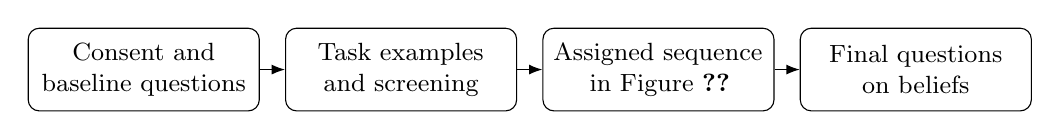
\begin{tikzpicture}[n/.style={draw,rounded corners,align=center,text width=2.7cm,minimum height=1.05cm,font=\small},>=Latex]
\node[n] (a) {Consent and\\baseline questions};
\node[n,right=.32cm of a] (b) {Task examples\\and screening};
\node[n,right=.32cm of b] (c) {Assigned sequence\\in Figure~\ref{fig:treeB}};
\node[n,right=.32cm of c] (d) {Final questions\\on beliefs};
\draw[->](a)--(b);\draw[->](b)--(c);\draw[->](c)--(d);
\end{tikzpicture}
\caption{\new{Common survey timeline. Professional characteristics precede the policy procedure; final belief reports follow the decisions. Policy ranking occurs at different points across arms.}}\label{fig:timelineB}
\end{figure}

\begin{figure}[!htbp]\centering\color{added}
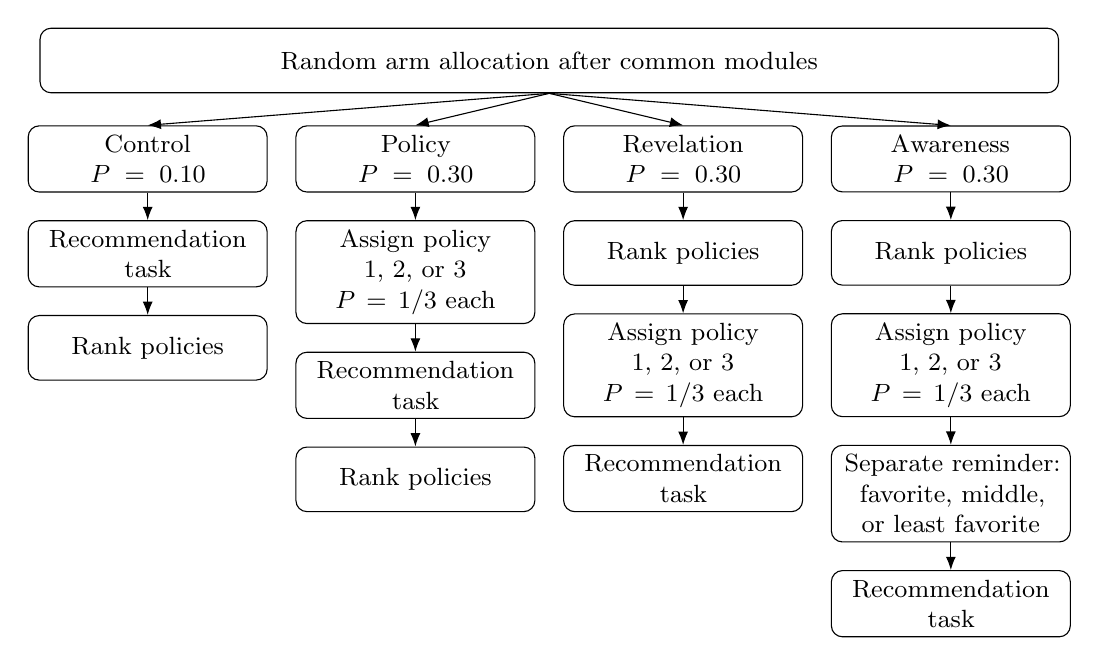
\begin{tikzpicture}[n/.style={draw,rounded corners,align=center,text width=2.8cm,font=\small,minimum height=.82cm},>=Latex]
\node[n,text width=12.7cm] (root) at (0,0) {Random arm allocation after common modules};
\node[n] (c) at (-5.1,-1.25) {Control\\$P=0.10$};
\node[n] (p) at (-1.7,-1.25) {Policy\\$P=0.30$};
\node[n] (r) at (1.7,-1.25) {Revelation\\$P=0.30$};
\node[n] (a) at (5.1,-1.25) {Awareness\\$P=0.30$};
\foreach \v in {c,p,r,a}{\draw[->](root.south)--(\v.north);}
\node[n,below=.35cm of c] (c1) {Recommendation\\task};
\node[n,below=.35cm of c1] (c2) {Rank policies};
\node[n,below=.35cm of p] (p1) {Assign policy\\1, 2, or 3\\$P=1/3$ each};
\node[n,below=.35cm of p1] (p2) {Recommendation\\task};
\node[n,below=.35cm of p2] (p3) {Rank policies};
\node[n,below=.35cm of r] (r1) {Rank policies};
\node[n,below=.35cm of r1] (r2) {Assign policy\\1, 2, or 3\\$P=1/3$ each};
\node[n,below=.35cm of r2] (r3) {Recommendation\\task};
\node[n,below=.35cm of a] (a1) {Rank policies};
\node[n,below=.35cm of a1] (a2) {Assign policy\\1, 2, or 3\\$P=1/3$ each};
\node[n,below=.35cm of a2] (a3) {Separate reminder:\\favorite, middle,\\or least favorite};
\node[n,below=.35cm of a3] (a4) {Recommendation\\task};
\foreach \u/\v in {c/c1,c1/c2,p/p1,p1/p2,p2/p3,r/r1,r1/r2,r2/r3,a/a1,a1/a2,a2/a3,a3/a4}{\draw[->](\u)--(\v);}
\end{tikzpicture}
\caption{\new{Vertical allocation and task sequence. Each treated policy cell has intended unconditional probability $0.30\times1/3=0.10$. The reminder is shown separately. Realized assigned and analyzed counts appear in Table~\ref{tab:flowB} and Appendix~\ref{app:cellsB}.}}\label{fig:treeB}
\end{figure}

\subsection{Policy content and recommendations}
The three scenarios are short descriptions of an educational environment under which teachers are asked to make their recommendations. Their English descriptions from the existing manuscript are retained in Appendix~\ref{app:policiesB}. Policy 1 promises small-group educational reinforcement with support staff. Policy 2 changes the evaluation-board procedure to unanimity for retention with secret and anonymous voting. Policy 3 provides tailored training and support in inclusive teaching and multilevel classroom management. No resources, evaluation-board voting rules, or staff training are actually implemented by assigning these descriptions.

The intended task presents eight student cards varying gender, complex background, failed subjects, basic competences, absence, and disciplinary problems. Each response recommends promotion or repetition. The existing inclusion rule excludes teachers recommending repetition for the favorable screening example. It does not exclude teachers declining repetition for the unfavorable example. We retain the established card coding and response sample: the two favorable-example fields are removed and other nonmissing recorded card responses are used. Most respondents therefore contribute eight or nine retained observations; some contribute fewer.

\new{This distinction matters more for treatment interpretation than for simple description. Introductory example responses precede assignment according to the study plan, and identifiers may be reused. The retained outcome is consequently a composite of collected recommendations, not a perfectly isolated mean of eight postassignment choices. An invariant preassignment component can dilute the measured treatment response; variable observation and profile composition can add further complications. We preserve the specified analysis rule but do not claim that profile adjustment recovers an unobserved postassignment-only outcome.}

\subsection{Analysis populations and outcome availability}
The raw export contains 4,942 records, including incomplete entries. Of these, 3,274 have an arm assignment: 337 Control, 984 Policy, 958 Revelation, and 995 Awareness. After the retained exclusion rules, 2,885 assigned records remain in the cleaned file, and 2,705 contribute a recommendation score. The remaining 180 retained assigned records have no usable recommendation. Table~\ref{tab:flowB} separates assignment, analytical retention, outcome availability, task-completion flags, and completion of the full survey.
\inputtab{added}{B_flow}{Assignment and availability of analysis outcomes}{tab:flowB}
\new{These indicators are not a single ordered survival sequence. Policy ranking is earlier in some arms, and a task-completion flag is not identical to retaining a usable outcome after exclusions. The assignment denominator is used for availability comparisons; rankings and final beliefs are not required for the main recommendation analysis. Ranking analyses use all retained respondents with the relevant ranking. In this export that rule produces the same 2,546 respondents as the intersection with score availability, but this equality is a property of the data rather than an imposed requirement.}

\section{Estimands and inference}
\subsection{Primary contrasts}
The main outcome is relative recommendation propensity. For teacher $j$, each recorded decision $Y_{ij}$ is compared with the leave-one-out repetition rate for the same card identifier, and these differences are averaged:
\[
 H_j=\frac{1}{n_j}\sum_{i\in I_j}(Y_{ij}-\bar Y_{i,-j}).
\]
The pooled reference standardizes for the cards observed. Multiplication by 100 expresses the result in percentage points. The main score sample does not condition on a policy ranking. A direct card-level analysis with card fixed effects and teacher-clustered errors provides a complementary specification.

The primary contrasts are Policy minus Control, Revelation minus Policy, and Awareness minus Revelation. The first compares an equally randomized mixture of the three assigned scenarios with no assigned scenario. The second changes ranking timing as well as prior exposure to all three policy descriptions. It is therefore the effect of that procedure, not an isolated effect of speaking a preference while holding information exposure constant. The third adds an explicit reminder after the same ranking-and-assignment sequence.

Unadjusted differences in teacher means are the primary estimates. Baseline-adjusted models use only the demographic and professional variables collected before the procedure. HC3 covariance accommodates heteroskedasticity at the teacher level. Teacher fixed effects cannot identify the main effect of an assignment that is constant within that teacher, so they are not added to these between-teacher regressions. There is no reliable school identifier for school-level clustering.

\new{Random assignment motivates intention-to-treat contrasts for an outcome observed for all assigned respondents. Here some outcomes are unavailable or excluded. The reported complete-observation differences follow assigned groups but are not automatically unbiased full-assignment ITT estimates. Their causal interpretation requires assumptions about selection and the recorded composite outcome. The availability comparisons, weighting sensitivity, and bounds below make this distinction explicit. A bootstrap with 399 teacher resamples reconstructs the profile reference, rather than treating the generated score as fixed throughout resampling.}

\subsection{Policy identities, preferences, and multiplicity}
We estimate the ten cell means and express all contrasts in a consistent direction. Within each treated arm, policies 2 and 3 are compared with policy 1. Within each policy, Revelation is compared with Policy and Awareness with Revelation. Two-by-three models provide joint tests of arm-by-policy interactions; additional joint tests compare the three policy identities within each arm. Individual contrast families use Holm adjustment \cite{holm}: three broad comparisons, nine treated cells versus control, six within-arm policy comparisons, and six between-arm comparisons within policy.

For Revelation and Awareness, preferences are elicited before policy assignment. We compare assignments to favorite and least-favorite policies against the middle-ranked policy, adjusting for favorite-policy identity, and test whether the reminder changes these contrasts. These estimates concern assignment to policy packages defined by prior rankings. Prior ranking does not randomize the underlying preference or separate policy content from alignment.

For Policy and Control, rankings follow the task. We retain the original ranking-adjusted and alignment-stratified specifications as secondary descriptions. Conditioning on a variable that may respond to assignment can change experimental comparisons \cite{post}. A small treatment coefficient on recommendations does not remove that concern. Later rankings are also analyzed as outcomes: for each policy, we compare the probability of ranking it first or last between respondents assigned to it and respondents assigned to another policy within the Policy arm, adjusting multiplicity over the six comparisons.

\subsection{Precision and selection sensitivity}
We distinguish two summaries of the precision of a contrast.
\old{The first is the minimum detectable effect with 80 percent power. This tells us which effect sizes the design was able to detect with reasonable probability. The second is an equivalence test. This asks whether we can reject effects outside a given substantive margin.}
In the present reanalysis, MDEs are approximate sensitivity summaries calculated from the realized standard errors, not a substitute for prospective power calculations. Equivalence uses two one-sided tests at five percent, equivalent to checking whether a 90 percent interval lies inside a specified margin \cite{equivalence}. We report margins of two, three, and five percentage points. These are transparent sensitivity thresholds, not retrospectively declared preregistered smallest effects of interest. Individual equivalence tests are not simultaneous guarantees across every policy and subgroup.

\new{Availability models compare the probability of retaining a score, task completion, and survey completion across assigned arms and policies. Alignment-related availability is examined only where rankings precede policy assignment. Baseline balance comparisons use age, gender, experience, stage, and ownership, which are potentially observed among both retained and missing-outcome respondents. Final belief reports cannot diagnose selection among respondents who never reach them.}

\new{Two further analyses assess sensitivity to selection. Inverse-observation weighting uses baseline variables and assigned arm, with median replacement and missingness indicators for baseline omissions. It assumes selection is ignorable conditional on that information and sufficient overlap. HC3 intervals in this exercise condition on estimated weights; it is a sensitivity check rather than a complete solution to estimated-selection uncertainty. Separately, worst-case bounds assign all missing outcomes either zero or one for the raw teacher-average binary recommendation measure. These require no missing-at-random assumption but concern a different outcome from $H_j$. We do not impose the monotonicity assumption required by Lee bounds across these procedures \cite{lee}.}

\section{Results}
\subsection{Average contrasts are small, with unequal precision}
Table~\ref{tab:broadB} reports the three primary comparisons. Policy minus Control is 0.62 points, with a 95 percent interval from $-2.27$ to 3.51. Revelation minus Policy is $-1.32$ points, with an interval from $-3.32$ to 0.67. Awareness minus Revelation is $-1.11$ points, with an interval from $-3.22$ to 1.00. None rejects a zero difference, with or without the broad-family multiplicity adjustment.
\inputtab{revised}{B_broad}{Primary recommendation contrasts and precision}{tab:broadB}
The three-point equivalence test yields a more discriminating conclusion. Policy versus Control does not pass: its 90 percent interval is [$-1.80$, 3.05] points. Revelation versus Policy passes narrowly, with [$-2.99$, 0.35], and Awareness versus Revelation passes with [$-2.88$, 0.66]. None of these three contrasts meets the tighter two-point margin; all meet the five-point margin under the primary HC3 specification. These are conditional observed-outcome conclusions, not evidence that all policy effects are exactly zero.
\plot{revised}{policy_broad}{Primary differences in relative recommendation propensity. Intervals are 95 percent; shading marks a three-point sensitivity margin. Equivalence decisions use 90 percent intervals.}{fig:broadB}
Baseline adjustment produces the same qualitative pattern of small estimates. Bootstrap 95 percent intervals rebuilding the score reference are [$-2.23$, 3.51], [$-3.39$, 0.73], and [$-2.98$, 1.01] points. These checks support describing the average estimates as small and imprecise around zero, but the close equivalence boundary for prior elicitation should not be presented as a robust qualitative separation between procedures.

\subsection{Policy-specific contrasts do not support a broad mechanism claim}
Figure~\ref{fig:cellsB} displays the ten mean outcomes; Table~\ref{tab:policiesB} groups the policy and arm contrasts. Policy 2 minus policy 1 within the Policy arm is approximately 2.13 points before conditioning on a later favorite ranking. The full pattern does not provide strong evidence of differences between policy identities: joint-test $p$-values are 0.423, 0.885, and 0.928 in Policy, Revelation, and Awareness. Joint arm-by-policy interaction tests give $p=0.785$ for Revelation versus Policy and $p=0.949$ for Awareness versus Revelation.
\plot{revised}{policy_cells}{Mean relative recommendation propensity in the ten assignment cells, with HC3 95 percent intervals. These are levels relative to pooled profile benchmarks, not differences from control.}{fig:cellsB}
\inputtab{revised}{B_policy_contrasts}{Policy identity and procedure comparisons}{tab:policiesB}
The ranking-adjusted specification for policy 2 yields Revelation minus Policy of $-3.04$ points (95 percent interval $-6.24$ to 0.15; unadjusted $p=0.062$). Its direction is toward lower, not higher, relative recommendation propensity under Revelation. Because the specification includes a ranking observed at different times, and the contrast is one among several, it cannot establish a mechanism of resistance or acceptance. The complete unadjusted cell comparisons are the clearer starting point for interpretation.

\subsection{Prior alignment and later preference reports answer different questions}
Among teachers who rank policies before assignment, favorite versus middle-ranked assignment is associated with 2.23 points in Revelation and 1.13 points in Awareness. Their 95 percent intervals are [$-1.05$, 5.51] and [$-2.31$, 4.57]. Least-favorite versus middle-ranked assignment gives 0.21 and 1.58 points, respectively, also with intervals spanning zero. The joint interaction test for changing these alignment contrasts with the reminder gives $p=0.583$. These comparisons do not tightly exclude all substantively relevant alignment responses.
\inputtab{added}{B_alignment}{Alignment using preferences elicited before policy assignment}{tab:alignB}
In contrast, reported preferences are not uniformly insensitive to assignment. Within Policy, 761 retained respondents provide a ranking. Assignment to teacher training raises its subsequent first-place ranking probability by 9.76 points, with a 95 percent interval from 2.50 to 17.01. The Holm-adjusted $p$-value is 0.0507 across six first/last-place outcomes. Its last-place ranking falls by 5.85 points, with an interval narrowly including zero. Table~\ref{tab:prefB} presents the complete family so that this finding is not selected in isolation.
\inputtab{revised}{B_preferences}{Assigned policy and its subsequent ranking in the Policy arm}{tab:prefB}
\new{The evidence is suggestive of a change in reported valuation or response consistency, but does not distinguish those mechanisms and does not survive a conventional five-percent Holm threshold. It is not necessary to establish a definitive ranking effect to recognize that a later ranking is potentially posttreatment. Conversely, the null average recommendation contrasts do not constitute a test of invariance in preferences.}

\subsection{Outcome availability and robustness delimit the interpretation}
The probability of observing a retained score is 83.38 percent in Control, 83.74 percent in Policy, 82.46 percent in Revelation, and 81.41 percent in Awareness. The corresponding adjacent-arm differences are 0.36, $-1.28$, and $-1.06$ points, with 95 percent intervals spanning zero. These similarities do not prove ignorable selection. Teachers with an observed retained score are younger than assigned respondents without one (45.06 versus 48.82 years) and have less experience (16.85 versus 20.24 years). These differences combine the retained screening rule and missing responses; they should not all be attributed to quitting the survey.

\new{Inverse-observation-weighted estimates are 0.64, $-1.27$, and $-1.15$ points, close to the primary results under the weighting assumptions. Symmetrically trimming the fastest and slowest 1.75 percent by total recorded duration also leaves small broad-arm estimates. Total duration may include time away from the survey, so trimming is a sensitivity analysis rather than a preferred attention rule. A direct card-level model with profile effects is reported in the appendix; its observation weighting differs from giving each teacher equal weight.}

The assumption-free bounds are much wider. For the raw mean recommendation outcome, Policy minus Control lies between $-15.54$ and 17.34 points under extreme assignments of missing outcomes; the other adjacent-arm bounds are [$-17.33$, 16.46] and [$-18.72$, 17.41]. These are identification bounds, not confidence intervals. Their width makes clear that similar observed availability rates do not establish small full-assignment effects without restrictions on the unobserved recommendations.

\section{Discussion}
The experiment yields small average changes in recorded recommendations when teachers receive a policy scenario, express policy preferences earlier, or receive an alignment reminder. The strongest interpretation is limited responsiveness of the observed composite outcome to these brief procedures, with differing precision across comparisons. It is weaker than a claim that educational policy does not matter, and more informative than simply listing nonsignificant hypotheses.

Policy scenarios operate through descriptions. The reinforcement scenario does not provide a support teacher; the training scenario does not change instructional skills; the unanimity scenario does not convene an evaluation board. A respondent may endorse a policy yet retain the same individual recommendation, especially when the policy would change collective decision rules rather than individual judgments. Actual implementation can affect behavior through resources, constraints, interactions, and learning that are absent here. The findings cannot be extrapolated to those channels.

The design also clarifies how preference elicitation enters an experiment. Moving ranking earlier both exposes respondents to the policy menu and asks them to order it before their decisions. The additional reminder makes an already elicited alignment explicit. Neither comparison alone identifies motivated reasoning. Small mean effects can reflect weak salience, heterogeneous responses, an unchanged decision threshold, limited understanding, or a genuine lack of response in this task. The data do not select a unique explanation.

Preferences observed at different times require different treatment. Prior preferences can define randomized policy-assignment contrasts within the relevant procedure, subject to selection. Later preferences can be informative outcomes or descriptive correlates, but should not be silently treated as baseline controls. The suggestive training-ranking result reinforces the practical importance of that distinction even though its multiplicity-adjusted evidence is borderline.

\new{The main limitations concern selection, measurement timing, and external validity. Approximately one sixth of assigned respondents lack a retained score. Some retained recommendations originate in examples, and the export does not separate every reused question instance. The sample is voluntary and regional; school-level dependence cannot be modeled reliably. Equivalence findings therefore apply to a defined recorded outcome under the stated inferential specification, not to all teachers, all policy identities, or a pure postassignment response.}

\new{A stronger follow-up would elicit baseline preferences comparably for all respondents, preserve distinct example and experimental response identifiers, measure comprehension, and observe outcomes after a more sustained or implemented intervention. Such a design could test whether weak responses arise from the brevity of the scenario, the content of the policy, or the alignment procedure. The present study identifies those separate questions and provides estimates around which a more informative replication can be designed.}

\section{Conclusion}
Brief policy scenarios and preference procedures produce small average contrasts in teachers' recorded repetition recommendations, but their effects are not uniformly equivalent to zero at a narrow margin. More specific policy and alignment comparisons remain uncertain, and selection limits full-assignment conclusions. Reporting these distinctions preserves what the experiment reveals: a measured response to hypothetical policy descriptions and preference procedures, rather than a test of whether implemented educational reforms can change retention.

\clearpage\begingroup\color{revised}\begin{thebibliography}{99}\small
\bibitem{allen} C. S. Allen, Q. Chen, V. L. Willson, and J. N. Hughes, ``Quality of research design moderates effects of grade retention on achievement: A meta-analytic, multilevel analysis,'' \textit{Educational Evaluation and Policy Analysis}, vol. 31, no. 4, pp. 480--499, 2009. \href{https://doi.org/10.3102/0162373709352239}{doi:10.3102/0162373709352239}.
\bibitem{goos} M. Goos, J. Pipa, and F. Peixoto, ``Effectiveness of grade retention: A systematic review and meta-analysis,'' \textit{Educational Research Review}, vol. 34, art. 100401, 2021. \href{https://doi.org/10.1016/j.edurev.2021.100401}{doi:10.1016/j.edurev.2021.100401}.
\bibitem{tomchin} E. M. Tomchin and J. C. Impara, ``Unraveling teachers' beliefs about grade retention,'' \textit{American Educational Research Journal}, vol. 29, no. 1, pp. 199--223, 1992. \href{https://doi.org/10.3102/00028312029001199}{doi:10.3102/00028312029001199}.
\bibitem{bonvin} P. Bonvin, ``The role of teacher attitudes and judgement in decision-making: The case of grade retention,'' \textit{European Educational Research Journal}, vol. 2, no. 2, pp. 277--294, 2003. \href{https://doi.org/10.2304/eerj.2003.2.2.6}{doi:10.2304/eerj.2003.2.2.6}.
\bibitem{klapproth} F. Klapproth and C. Beyte, ``GPA, student gender, school subject, and teacher attitudes in grade retention decisions: An experimental study,'' \textit{European Journal of Psychology of Education}, vol. 41, art. 24, 2026. \href{https://doi.org/10.1007/s10212-026-01072-7}{doi:10.1007/s10212-026-01072-7}.
\bibitem{kunda} Z. Kunda, ``The case for motivated reasoning,'' \textit{Psychological Bulletin}, vol. 108, no. 3, pp. 480--498, 1990. \href{https://doi.org/10.1037/0033-2909.108.3.480}{doi:10.1037/0033-2909.108.3.480}.
\bibitem{pajares} M. F. Pajares, ``Teachers' beliefs and educational research: Cleaning up a messy construct,'' \textit{Review of Educational Research}, vol. 62, no. 3, pp. 307--332, 1992. \href{https://doi.org/10.3102/00346543062003307}{doi:10.3102/00346543062003307}.
\bibitem{spillane} J. P. Spillane, B. J. Reiser, and T. Reimer, ``Policy implementation and cognition: Reframing and refocusing implementation research,'' \textit{Review of Educational Research}, vol. 72, no. 3, pp. 387--431, 2002. \href{https://doi.org/10.3102/00346543072003387}{doi:10.3102/00346543072003387}.
\bibitem{holm} S. Holm, ``A simple sequentially rejective multiple test procedure,'' \textit{Scandinavian Journal of Statistics}, vol. 6, no. 2, pp. 65--70, 1979. \url{https://www.jstor.org/stable/4615733}.
\bibitem{post} J. M. Montgomery, B. Nyhan, and M. Torres, ``How conditioning on posttreatment variables can ruin your experiment and what to do about it,'' \textit{American Journal of Political Science}, vol. 62, no. 3, pp. 760--775, 2018. \href{https://doi.org/10.1111/ajps.12357}{doi:10.1111/ajps.12357}.
\bibitem{equivalence} D. Lakens, ``Equivalence tests: A practical primer for t tests, correlations, and meta-analyses,'' \textit{Social Psychological and Personality Science}, vol. 8, no. 4, pp. 355--362, 2017. \href{https://doi.org/10.1177/1948550617697177}{doi:10.1177/1948550617697177}.
\bibitem{lee} D. S. Lee, ``Training, wages, and sample selection: Estimating sharp bounds on treatment effects,'' \textit{Review of Economic Studies}, vol. 76, no. 3, pp. 1071--1102, 2009. \href{https://doi.org/10.1111/j.1467-937X.2009.00536.x}{doi:10.1111/j.1467-937X.2009.00536.x}.
\end{thebibliography}
\endgroup
\clearpage\appendix
\section{Policy descriptions}\label{app:policiesB}
The following English descriptions preserve the wording in the existing manuscript. Numeric labels in the analysis correspond to A, B, and C respectively.
\begin{enumerate}
\item \old{\textbf{Policy A: Educational reinforcement.} The student will receive educational reinforcement in a small group next school year, with a support teacher, inside or outside the classroom.}
\item \old{\textbf{Policy B: Modified promotion criteria.} The promotion criteria will be modified in the Evaluation Board: unanimity for grade retention, secret and anonymous voting.}
\item \old{\textbf{Policy C: Teacher training.} All school staff will receive tailored training and teaching support in inclusive teaching methodologies and multi-level classroom management.}
\end{enumerate}
\new{The questionnaire asks respondents to rank the three policies from favorite to least favorite. The initial display order is randomized according to the study plan. In Awareness, the reminder reports whether the assigned policy occupies the favorite, middle, or least-favorite position. The relevant intervention is the presence of this reminder, conditional on the earlier assigned arm; its content is not a separately randomized treatment.}

\section{Cell counts, availability, and selection}\label{app:cellsB}
\inputtab{added}{B_cells_flow}{Realized policy-cell sample sizes}{tab:cellflowB}
\begin{addition}
The assignment universe is defined by a nonmissing valid treatment code in the raw export, not by completion of the final page. Screening retention, availability of a score, ranking availability, and the survey-finished flag are retained as separate indicators. Table~\ref{tab:availabilityB} shows availability contrasts from this universe. Comparisons of attrition by alignment are restricted to Revelation and Awareness respondents with an earlier ranking; they do not condition on later rankings from Policy. Conditional denominators for those contrasts are documented in the aggregate replication tables.
\end{addition}
\inputtab{added}{B_availability}{Differences in retained-score availability from assignment}{tab:availabilityB}
\inputtab{added}{B_balance}{Baseline characteristics by retained-score availability}{tab:balanceB}
\plot{added}{availability_by_arm}{Availability of recorded indicators relative to initial assignment. Connecting lines facilitate comparison of indicators; they are not survival curves, because ranking occurs at different points across arms.}{fig:availabilityB}
\new{The replication package contains all policy-by-arm and prior-alignment availability regressions, with their own denominators. Availability outcomes are not collapsed into a Cox model because task order differs across arms and total elapsed time is not a consistent measure of time at risk. Identification bounds use the observed fraction $r_a$ and observed mean $\bar Y_a$ in arm $a$: the arm mean is bounded by $[r_a\bar Y_a,r_a\bar Y_a+1-r_a]$. A difference takes the lower endpoint of one arm minus the upper endpoint of the other, and conversely.}

\section{Alternative specifications and precision}
\inputtab{revised}{B_sensitivity}{Primary contrasts under alternative specifications}{tab:sensB}
The card-level specification includes card fixed effects and clusters errors by teacher. It gives more weight to teachers with more recorded responses, unlike the teacher-level mean comparison. The baseline-adjusted specification conditions on professional characteristics observed before the policy procedure. Neither includes teacher fixed effects for the main assignment contrast. Bootstrap draws resample teachers and reconstruct leave-one-out profile rates. These procedures examine different sources of sensitivity and should not be interpreted as independent replications.
\inputtab{added}{B_equivalence}{Equivalence sensitivity for the broad-arm contrasts}{tab:eqB}
\new{The minimum detectable effects in Table~\ref{tab:broadB} use $(t_{.975}+t_{.80})\widehat{SE}$, approximately, for two-sided five-percent testing. They describe realized precision. Equivalence margins are expressed on the recommendation-probability scale: a three-point margin is neither three percent of the baseline rate nor three percent of a standard deviation. The family-specific Holm corrections apply to difference tests; individual equivalence conclusions are reported separately and do not certify that every subgroup is equivalent.}

\section{Secondary alignment and ranking-adjusted analyses}
\inputtab{revised}{B_secondary_alignment}{Secondary comparisons conditioning on reported alignment}{tab:secondaryB}
These specifications retain the original comparative structure, including comparisons to Control for favorite and least-favorite assignments in Policy and comparisons across successive arms within alignment categories. Where a ranking follows assignment or decisions, they are descriptive rather than the primary causal contrasts. The preferred temporal comparison for the reminder uses Revelation and Awareness with their preassignment ranking and the joint interaction test reported in the main text.

\section{Scope, plan, and replication disclosure}
\begin{addition}
The companion manuscript \textit{The Decision to Hold Back: Student Information, Teacher Disagreement, and the Limits of Predictability} uses the same survey to study within-teacher attribute patterns, same-profile disagreement, and held-out prediction. The present paper does not claim those results as a separate contribution. Editors and readers should evaluate the overlap with that shared dataset disclosed.

The local initial analysis plan describes the treatment structure and hypothesis families. The current organization, main sample definitions by objective, multiplicity summaries, selection diagnostics, and precision sensitivity analyses are part of a subsequent reanalysis. A public time-stamped registration is not asserted on the basis of the local PDF alone. The analysis scripts and aggregate outputs accompany the working manuscripts in a separate directory; the original manuscript and its results are preserved. Research-governance and data-release declarations require verification from the study records before journal submission.
\end{addition}
\end{document}


